\documentclass{article}
\usepackage{graphicx} % Required for inserting images
\usepackage[export]{adjustbox}
\usepackage{amsmath}
\usepackage{listings}
\usepackage{color}
\usepackage{tabularray}
\usepackage{hyperref}

\definecolor{dkgreen}{rgb}{0,0.6,0}
\definecolor{gray}{rgb}{0.5,0.5,0.5}
\definecolor{mauve}{rgb}{0.58,0,0.82}

\lstset{
frame=tb,
language=C,
aboveskip=3mm,
belowskip=3mm,
showstringspaces=false,
columns=flexible,
basicstyle={\small\ttfamily},
numbers=none,
numberstyle=\tiny\color{gray},
keywordstyle=\color{blue},
commentstyle=\color{dkgreen},
stringstyle=\color{mauve},
breaklines=true,
breakatwhitespace=true,
tabsize=3
}

\title{Algoritmo parallelo per il prodotto matrice-matrice}
\author{Puggioni Riccardo, Regina Riccardo, Trotti Francesco }
\date{December 2023}

\begin{document}

\maketitle

\newpage
\tableofcontents

\newpage
\section{Introduzione al problema}
    \subsection{Prodotto matrice-matrice}
Il prodotto matrice-matrice è un algoritmo dell'algebra lineare che definisce la moltiplicazione tra due matrici. Esso produce una nuova matrice.
Formalmente, sia $A \in M_{m,n}, B \in M_{n,p}$, allora $A\cdot B = C$, dove $C \in M_{m,p}$.
La matrice risultante $C$ viene calcolato dal seguente algoritmo:
\begin{lstlisting}
for i from 0 to m do
    for j from 0 to n do
        C[i][j] = scalarProduct(A, B, i, j);
\end{lstlisting}
dove scalarProduct(A, B, i, j) é l'algoritmo per il prodotto scalare standard tra l'$i$-esima riga di A e la $j$-esima colonna di B.

\subsection{Approccio alla risoluzione}
La suddivisione del carico di lavoro sfrutterá la libreria openMPI, che implementa il message passing tra calcolatori di tipo MIMD a memoria distribuita.

Verrá supposto che le matrici A e B siano quadrate e di eguale dimensione. Inoltre, considereremo esclusivamente i casi in cui il numero di processi sia un divisore della dimensione delle matrici.

\subsection{Strategia di comunicazione}
Per l'algoritmo del prodotto matrice-matrice, sono possibili tre tipi di suddivisione del carico.
\begin{enumerate}
    \item Si suddivide la matrice A in blocchi di righe, B in blocchi di colonne.
    \item Si suddivide A in blocchi di colonne, B in blocchi di righe.
    \item Si suddividono A e B in blocchi di colonne.
    \item Si suddividono A e B in blocchi quadrati.
\end{enumerate}
Tra queste, é stata scelta la quarta, anche nota come algoritmo di Fox o BMR (Broadcast Multiply Roll).

In primis, disponiamo virtualmente i processi secondo una topologia a griglia. Adesso, un processo avrá un indice di riga e di colonna.

Dividiamo le matrici in blocchi quadrati: verranno create delle sottomatrici $A_{ij}$, $B_{ij}$, $C_{ij}$, che verranno assegnate ai processi in posizione $ij$ nella griglia.

Supponiamo di avere una griglia 3x3 di processi. Allora ciascuna matrice (A,B,C) verrá suddivisa in 9 sottomatrici.

Le sottomatrici di C potranno essere calcolate con le seguenti operazioni:
$C_{00} = A_{00}\cdot B_{00} + A_{01}\cdot B_{10} + A_{02}\cdot B_{20}$ \\
$C_{01} = A_{00}\cdot B_{01} + A_{01}\cdot B_{11} + A_{02}\cdot B_{21}$ \\
$C_{02} = A_{00}\cdot B_{02} + A_{01}\cdot B_{12} + A_{02}\cdot B_{22}$ \\
... \\
$C_{22} = A_{20}\cdot B_{02} + A_{21}\cdot B_{12} + A_{22}\cdot B_{22}$ \\


\begin{figure}[!htbp]
    \centering
    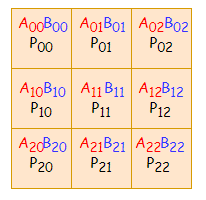
\includegraphics{distribuzioneIniziale.png}
    \caption{Distribuzione iniziale dei sottoblocchi di A e B}
    \label{fig:enter-label}
\end{figure}  
\begin{figure}[!htbp]
    \centering
    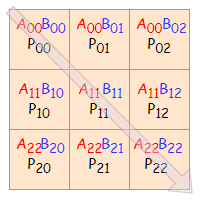
\includegraphics{primaDiagonale.png}
    \caption{Primo passo}
    \label{fig:enter-label}
\end{figure}  
\begin{figure}[!htbp]
    \centering
    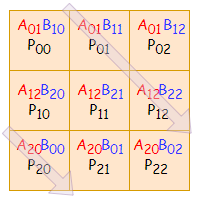
\includegraphics{secondaDiagonale.png}
    \caption{Secondo passo}
    \label{fig:enter-label}
\end{figure}  
\begin{figure}[!htbp]
    \centering
    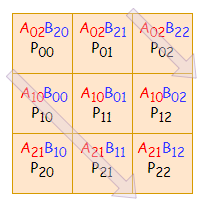
\includegraphics{terzaDiagonale.png}
    \caption{Terzo passo}
    \label{fig:enter-label}
\end{figure}  

Notiamo che, con questa disposizione delle sottomatrici, solo i processi sulla diagonale maggiore riusciranno a calcolare un contributo per la propria sottomatrice C di competenza. In particolare, notiamo che tutti i processi sulla stessa riga necessitano del sottoblocco B dell'elemento sulla diagonale. Quindi, condividiamo tale sottoblocco con tutti i processi sulla stessa riga, che adesso potranno calcolare un addendo della propria sottomatrice C.

Successivamente, notiamo che un processo in posizione i,j della griglia puó calcolare un altro addendo: 
\begin{itemize}
    \item richiedendo il sottoblocco B dal processo in posizione i-1,j, considerando peró la periodicitá delle dimensioni ($0 - 1 = 2$). Allora, effettuiamo una rotazione verticale verso l'alto dei sottoblocchi di B.
    \item richiedendo il sottoblocco A dal processo che si trova sulla diagonale che parte dalla posizione 01 (diagonale maggiore shiftata di 1 elemento verso destra). Quindi condividiamo tale sottoblocco con i processi della stessa riga.
\end{itemize}


Per calcolare l'ultimo addendo, dovremmo ripetere il passo precedente, ma shiftando un altra volta di una posizione verso destra la diagonale di riferimento.

A questo punto, avendo capito il pattern, generalizziamo l'algoritmo:
\begin{lstlisting}
    for k from 0 to p-1 do
        //controllo se sono un processo sulla diagonale attuale
        if coord_x = (coord_y-k)mod p then
            broadcast A_local to x-th row processes
        else
            receive into A_local_temp from process in position (coord_x, (coord_x+k)mod p)

        //effettuo il calcolo locale
        C_local = C_local + matrixProduct(A_local_temp, B_local)

        //ruoto verticalmente B
        send B_local to process in position ((coord_x-1)mod p, coord_y)
        receive into B_local from process in position ((coord_x+1)mod p, coord_y)
\end{lstlisting}

\section{Implementazione dell'algoritmo}
    \subsection{Header file richiamati}
\begin{lstlisting}
#include <omp.h>
#include <stdio.h>
#include <stdlib.h>
\end{lstlisting}

\subsection{Main}
Nel blocco del main, ovvero il punto di ingresso del programma, viene in primis effettuata la dichiarazione della matrice $A$ e delle sue dimensione $m$, $n$, del vettore $x$ di dimensione $dim$.
Viene controllato se $dim$ e $n$ coincidano, ovvero se il prodotto è ben definito.
A questo punto, se il controllo è andato  a buon fine, viene chiamata la funzione centrale del programma.
Infine, viene eseguita la stampa del vettore $y$ risultante.

\begin{lstlisting}
int main(){
    int m, n;
    double **A = readMatrixFromFile("<path>", &m, &n);

    int dim;
    double *x = readVector("<path>", &dim);

    if(dim != n){
        printf("Vettore e matrice non hanno dimensioni adeguate per una moltiplicazione...");
        exit(-1);
    }
    
    double *y = matrixVector(m, n, x, A);
    printVector(y, m);

    return 0;
}
\end{lstlisting}

\subsection{Algoritmo}
La direttiva omp \textit{\#pragma} indica l'inizio di un blocco parallelo: il master thread (nato alla nascita del processo) genera un team di thread, sottoprocessi che condividono la stessa area di memoria. Pertanto, è importante specificare ai thread quali saranno le variabili condivise, accessibili a tutti e regolate da un semaforo di sistema, e quali private, sempre sovrascrivibili perché indipendenti. 

Per decidere manualmente la visibilitá delle variabili é stata usata la direttiva \textit{default(none)}.
Le variabili condivise sono: gli indirizzi di memoria della matrice A ($A$) e dei vettori ($x$ e $y$); le rispettive dimensioni ($m$, $n$) e ($n$, $m$), che devono poter essere visualizzate in ogni istante della computazione da ciascun thread.
Le variabili private sono gli indici dei due cicli for innestati. Ogni thread compierà le proprie iterazioni indipendenti.
Per la distribuzione delle iterazioni del for-statement, si è usata una specifica direttiva  standard di omp: \textit{\#pragma...for...}. 
La fine del for-statement sancisce anche la fine della regione parallela: si verifica il ricongiungimento dei thread nel master thread.
La funzione infine restituirà al main l'indirizzo di memoria del vettore risultante $y$.
\begin{lstlisting}
double *matrixVector(int m, int n, double *x, double **A){
    
    double *y = calloc(m, sizeof(double));
    int i, j;
    #pragma omp parallel for default(none) shared(m,n,x,A,y) private(i,j)
        for (i = 0; i < m; i++){
            for (j = 0; j < n; j++){
                y[i] += A[i][j] * x[j];
            }
        }
    return y;
}
\end{lstlisting}

\subsection{Funzioni accessorie}
Mostriamo adesso le altre funzioni utilizzate nel blocco del main.
\subsubsection{Lettura da file della matrice e del vettore}
\begin{lstlisting}
double **readMatrixFromFile(char *path, int *m, int *n){
    FILE *fp;
    fp = fopen(path,"r");
    int i,j;

    fscanf(fp, "%d %d", m, n);

    double **A = malloc((*m) * sizeof(double *));
    for (i = 0; i < (*m); i++)
        A[i] = malloc((*n) * sizeof(double));

    
    for (i = 0; i < (*m); i++){
        for (j = 0; j < (*n); j++){
            fscanf(fp, "%lf", &(A[i][j]));
        }
    }

    fclose(fp);
    return A;
}
\end{lstlisting}

\begin{lstlisting}
double *readVector(char *path, int *m){
    FILE *fp;
    fp = fopen(path,"r");
    int i;
    fscanf(fp, "%d", m);

    double *x = malloc((*m) * sizeof(double));

    for(i = 0; i < (*m); i++){
        fscanf(fp, "%lf", x+i);
    }
    fclose(fp);
    return x;
}
\end{lstlisting}

\subsubsection{Stampa del vettore risultante}
\begin{lstlisting}
void printVector(double *y,int m){
    int i;
    for(i = 0; i < m; i++){
        printf("%f ", y[i]);
    }
    printf("\n");
}
\end{lstlisting}



\section{Analisi dei tempi di esecuzione}
    \subsection{Tempo di esecuzione}

Nel calcolare il tempo di esecuzione di un algoritmo parallelo, la grandezza nota come complessità di tempo (utile nell'analisi del tempo di esecuzione di un algoritmo sequenziale) risulta poco indicativa.\\
Infatti, in un algoritmo parallelo il numero delle operazioni non coincide più con il numero dei passi temporali. Di conseguenza si introducono nuove grandezze al fine di realizzare un'analisi degli algoritmi paralleli.

Adattando i concetti del calcolo parallelo in calcolatori MIMD a memoria distribuita a quelli a memoria condivisa: se T che indica il numero di thread eseguibili parallelamente dai core della macchina, un problema che si risolve in un tempo t verrà risolto da T thread (idealmente) in $\frac{t}{T}$.

\subsection{Speed-up, Overhead ed Efficienza}

Lo \textbf{speed-up} misura la riduzione del tempo di esecuzione rispetto all'algoritmo sequenziale ed è definito dal rapporto:
$$ S(T) = \frac{t(1)}{t(T)} $$ 

La quantità che misura quanto il nostro speed up differisce da quello ideale è l'overhead. Si può quantificare con la seguente formula: $O_h(T) = T\cdot t(T) - t(1)$ .\\
Riscrivendo lo speed up in funzione dell'overhead ci accogiamo infatti che lo speed up è ideale se e solo se l'overhead è nullo.\\

Per poter misurare se e quanto è stato "sfruttato" il nostro ambiente di calcolo parallelo, si introduce l' \underline{efficienza} del nostro algoritmo.
Si definisce \textbf{efficienza} il rapporto: $$ E(T) = \frac{S(T)}{T} $$

\subsection{Modifiche al codice per la registrazione dei tempi}
\subsubsection{Header file}
Il linguaggio C fornisce un tipo built-in per gestire la grandezza fisica del tempo: time.
La sua definizione é contenuta nel file header che segue e che pertanto deve essere incluso nel codice sorgente:
\begin{lstlisting}
#include <sys/time.h>
\end{lstlisting}

\subsubsection{Main}
Il main delega il calcolo dell'effettivo algoritmo all'algoritmo stesso, passando la variabile time alla funzione matrixVector.
La variabile numThreads é invece un discriminante per l'analisi finale dei dati.
Sia time che numThreads verranno modificate a runtime dalla funzione matrixVector.
Infine, invochiamo writeResultOnFile per registrare il risultato ottenuto.
\begin{lstlisting}
    int main(){
        double time;
        int numThreads;

        int m, n;
        double **A = readMatrixFromFile("<path>", &m, &n);
    
        int dim;
        double *x = readVector("<path>", &dim);
    
        if(dim != n){
            printf("Vettore e matrice non hanno dimensioni adeguate per una moltiplicazione...");
            exit(-1);
        }
        
        double *y = matrixVector(m, n, x, A, &time, &numThreads);
        printVector(y, m);
        writeResultOnFile("results.txt", m, n, time, numThreads);
        printf("execution time--->%.10lf", time);
    
        return 0;
    }
\end{lstlisting}

\subsubsection{Algoritmo}
La variabile numThreads viene inizializzata con il valore restituito dalla funzione omp_get_max_threads(), una funzione della libreria omp che restituisce il massimo numero di thread disponibili per la successiva regione parallela.
Ai fini del calcolo del tempo d'esecuzione, ci serviamo della funzione gettimeofday, che restituisce un oggetto di tipo struct timeval, contenente il clock, il giorno di sistema ed altre informazioni.
Alla prima chiamata a gettimeofday, salviamo il valore in secondi nella variabile timeStart, mentre alla seconda, salviamo in timeEnd.
L'istruzione "t.tv_sec+(t.tv_usec / 1000000.0)" somma i secondi conservati da t ai microsecondi conservati da t divisi per 1000000 (i microsecondi vengono riscalati a secondi).
Assegniamo al parametro time il la differenza tra timeEnd e timeStart.
\begin{lstlisting}
    double *matrixVector(int m, int n, double *x, double **A, double *time, int *numThreads){
        (*numThreads) = omp_get_max_threads();
    
        struct timeval t;
        gettimeofday(&t, NULL);
        double timeStart = t.tv_sec+(t.tv_usec / 1000000.0);

        double *y = calloc(m, sizeof(double));
        int i, j;
        #pragma omp parallel for default(none) shared(m,n,x,A,y) private(i,j)
            for (i = 0; i < m; i++){
                for (j = 0; j < n; j++){
                    y[i] += A[i][j] * x[j];
                }
            }

        gettimeofday(&t, NULL);
        double timeEnd = t.tv_sec+(t.tv_usec / 1000000.0);

        (*time) = timeEnd - timeStart;

        return y;
    }
\end{lstlisting}

\subsubsection{Scrittura dei tempi raccolti}
Segue la definizione della funzione invocata alla fine del main: writeResultOnFile.
\begin{lstlisting}
    void writeResultOnFile(char *path, int m, int n, double time, int numThreads){
        FILE *fp;
        fp = fopen(path,"a");

        fprintf(fp, "Dimensione in Input: %dx%d \nTempo di esecuzione: (%.10lf secondi) \nNumero di thread nel team: %d\n\n\n", m, n, time, numThreads);
        fclose(fp);
    }
\end{lstlisting}

\subsection{Dati empirici}
L'algoritmo è stato testato in più condizioni e secondo i parametri precedentemente descritti.
É stato fissata una dimensione di 1000x1000 per la matrice in input e di 1000 per il vettore.
Il numero di thread é variato da 1 a 8, tenendo conto delle sole potenze di 2.

\begin{table}[htp]
\centering
%\caption{}
\begin{tblr}{
  hlines,
  vlines,
}
Threads & Tempo ($\cdot 10^{-3} s$) & Speed Up & Efficienza & Overhead ($\cdot 10^{-3} s$) \\
1          & x   & x    & x       & x                     \\
2          & x   & x    & x       & x                     \\
4          & x   & x    & x       & x                     \\
8          & x   & x    & x       & x                     
\end{tblr}
\end{table}


\clearpage

Il grafico dei tempi:
\begin{figure}[h!tbp]
    \centering
    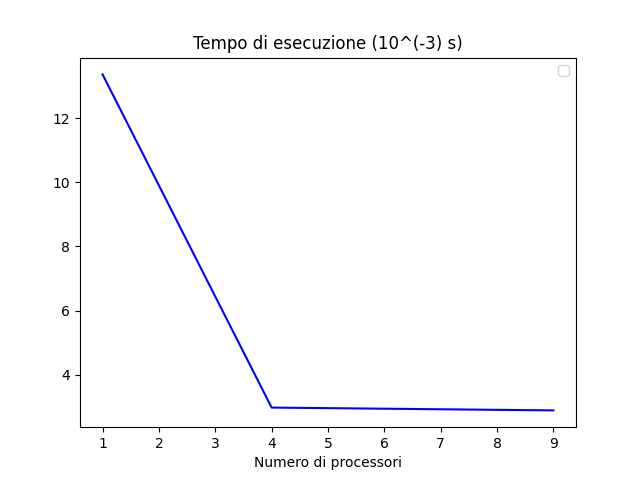
\includegraphics[width=1\linewidth]{Tempi.png}
    \caption{Andamento dei tempi}
    \label{fig:enter-label}
\end{figure}

\newpage
Visualizziamo la curva, confrontandola all'andamento dello speed-up ideale:
\begin{figure}[h!tbp]
    \centering
    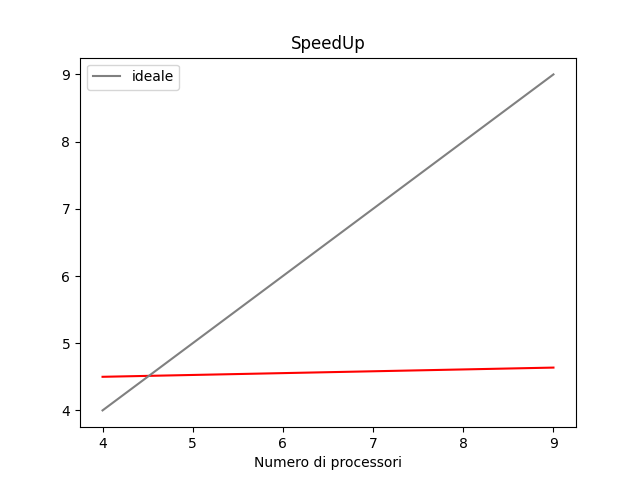
\includegraphics[width=1\linewidth]{SpeedUp.png}
    \caption{Andamento dello Speed Up}
    \label{fig:enter-label}
\end{figure}
\clearpage
Visualizziamo su un grafico anche i valori dell'Overhead:

\begin{figure}[h!tbp]
    \centering
    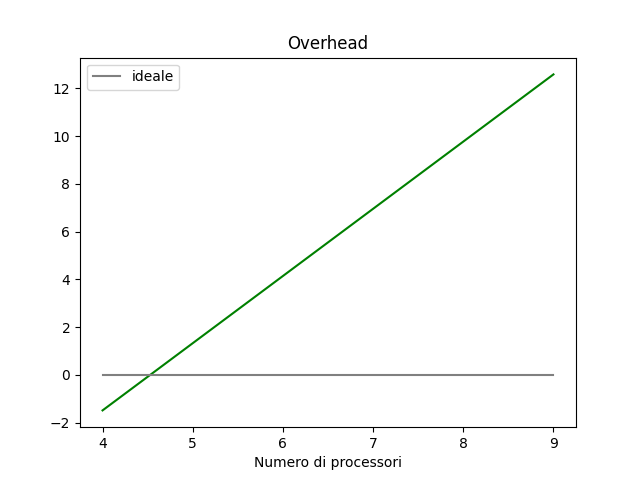
\includegraphics[width=1\linewidth]{Overhead.png}
    \caption{Andamento dell'Overhead}
    \label{fig:enter-label}
\end{figure}

\clearpage

Infine osserviamo come varia la nostra efficienza:
\begin{figure}[h!tbp]
    \centering
    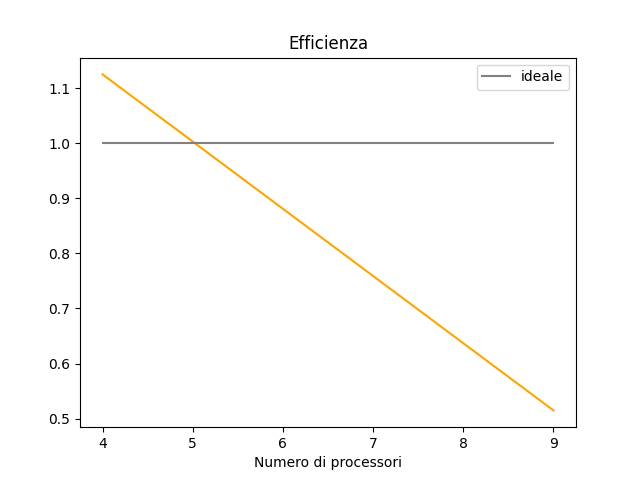
\includegraphics[width=1\linewidth]{Efficienza.png}
    \caption{Andamento dell'efficienza}
    \label{fig:enter-label}
\end{figure}

\section{Modalità d'uso}
    Il programma deve essere eseguito mediante un job script contenente direttive pbs (portable batch system).

Un esempio di jobscript:
\begin{lstlisting}
INSERIRE SCRIPT PER OMP
\end{lstlisting}

Una volta scritto il job script, per eseguirlo, bisognerà eseguire da terminale il comando 
\begin{lstlisting}
qsub FILE.pbs
\end{lstlisting}

In caso l'esecuzione dello script vada a buon fine, verranno generati FILE.out e FILE.err, i file di output e errore rispettivamente.

Per andare a visualizzare tali file, bisognerà eseguire da terminale i comandi
\begin{lstlisting}
cat FILE.err
cat FILE.out
\end{lstlisting}

\section{Esempi d'uso}
    %In algebra lineare, il prodotto matrice-vettore puó rappresentare il calcolo dell'immagine di un vettore mediante un applicazione lineare.
Le applicazioni lineari sono fondamentali in alcuni settori notevoli della scienza odierna, come:
\begin{itemize}
    \item le reti neurali e il deep learning.
    \item il machine learning: nella regressione lineare il prodotto matrice-vettore calcola l'output previsto.
    \item la compressione e la codifica dei video: nell'algoritmo MPEG, il prodotto matrice-vettore viene utilizzato per ridurre la dimensione del video.
    \item la grafica digitale.
\end{itemize}
Dunque massimizzare la sua efficienza é alla base dell'efficientamento delle tecnologie menzionate di sopra.

\end{document}